\chapter[Metodologia]{Metodologia}

Essa seção é dividida em dois grandes blocos, que elucidam duas grandes etapas do projeto. Primeiramente, tem-se a prova de conceito, no qual fluxogramas visam explanar a lógica de funcionamento, apontando qual é a entrada e a saída daquele bloco, bem como, qual é o processamento realizado. A prova de conceito foi implementada em um \textit{software} de síntese musical chamado \textit{PureData}.


Em seguida, encontra-se a seção da implementação final realizada. Essa seção é divivida em duas subseções: uma dedicada ao \textit{hardware}, que explica como os sinais de controle foram obtidos e como o sinal de saída se dá para que possa ser reproduzido em um sistema de som, e outra dedicada ao \textit{software}, que engloba a aquisição do sinal através de arquivos de música no formato \textit{.wav}, explicações de aquisição de sinais analógicos convertidos para digitais, que são responsáveis pelos controles de frequência, escolha do efeito e a quantidade de efeito aplicado, além do processo de construção do filtro utilizado na aplicação.

\section{Proposta Geral}

A evolução dos equipamentos de mixagem começou com a mixagem em vinil, e ao longo do tempo, novas funcionalidades foram adicionadas, como o \textit{jogger} para atraso e avanço da música, \textit{fader} para controle de volume e \textit{knobs} para ajuste de frequências. Com o avanço da microeletrônica, esses equipamentos evoluíram para a eletrônica digital, incorporando \textit{DSPs} para processar formatos de áudio de alta qualidade, como WAV e FLAC.

Atualmente, existem dois tipos principais de equipamentos de mixagem: os mais caros, que não requerem um computador, e os mais acessíveis, que dependem de um computador, mas oferecem melhor qualidade de processamento. DJs iniciantes frequentemente enfrentam dificuldades para realizar ajustes finos nas bandas de frequência em \textit{mixers} clássicos de três bandas. Esta habilidade é crucial para destacar elementos musicais e criar novas atmosferas. À medida que um DJ desenvolve seu estilo, a mixagem torna-se mais automática, facilitando a transição entre músicas.

Este projeto propõe a criação de um \textit{mixer} com um controle central que manipula dois arquivos de música. Em vez dos tradicionais controles de três bandas de frequência, o \textit{mixer} utilizará filtros passa-altas. O controle central ajustará simultaneamente as frequências de corte de ambos os canais, permitindo uma transição suave entre as músicas.

Além disso, o sistema incluirá dois efeitos, \textit{delay} e \textit{reverb}, que serão controlados através de um botão giratório, que determinará a intensidade do efeito aplicado.

Em resumo, o sistema processará arquivos de áudio que já estejam dentro da \textit{Raspberry Pi}, utilizando filtros passa-altas e permitindo ao usuário selecionar e controlar a intensidade dos efeitos, com botões \textit{knobs} para ajuste e um botão \textit{on}/\textit{off} para seleção dos efeitos.

\section{Levantamento de Requisitos}

O levantamento de requisitos é uma etapa crucial no desenvolvimento de qualquer sistema, pois define as funcionalidades e características necessárias para atender às necessidades dos usuários finais. Nesta seção, são apresentados os requisitos funcionais e não funcionais, que especificam o comportamento esperado do sistema, assim como as restrições e qualidades que devem ser atendidas. Os requisitos foram organizados em categorias que abrangem desde aspectos de desempenho e interface do usuário até segurança e manutenção, assegurando uma visão completa e detalhada do que o sistema deve entregar.

\subsection{Requisitos Funcionais}

Nessa subseção, são levantados os requisitos que descrevem o que o sistema deve realizar, bem como funcionalidades e comportamentos.
\begin{itemize}
    \item O sistema deve permitir ao \textit{DJ} utilizar arquivos \textit{.wav}.
    \item O sistema deve permitir ao \textit{DJ} controlar a frequência de corte.
    \item O sistema deve permitir ao \textit{DJ} controlar a presença dos efeitos.
\end{itemize}

\subsection{Requisitos Não Funcionais}
Já nesta subseção, há a descrição de como o sistema deve se comportar em relação ao desempenho, segurança, usabilidade e outros atributos qualitativos.  
\begin{itemize}
    \item O sistema deve responder aos comandos do \textit{DJ} com latência mínima, garantindo uma experiência de mixagem fluida.
    \item O sistema deve ser confiável e estável, capaz de lidar com longos períodos de uso contínuo sem falhas.
    \item O sistema deve oferecer uma qualidade de som de alta fidelidade, garantindo que o áudio reproduzido seja claro e com mínimas distorções.
    \item A interface do mixer deve incluir botões físicos ou controles táteis para ajuste de frequência e efeitos de áudio.
    \item A interface do mixer deve ser organizada de forma lógica e intuitiva, com controles agrupados por função para facilitar a navegação.
    \item A interface deve possuir indicações claras das funções dos botões de interação com o usuário.
    \item O sistema deve incluir interface de saída de áudio padrão \textit{RCA}.
    \item O sistema deve suportar uma ampla gama de frequências de áudio, garantindo que os graves sejam reproduzidos com profundidade e os agudos sejam nítidos e claros.
    \item O sistema deve ser projetado para minimizar o risco de danos aos equipamentos de áudio conectados.
\end{itemize}



\section{Fluxograma do Mixer}

O \textit{mixer} proposto é composto por sub-blocos de funcionamento interligados, conforme ilustrado na Figura \ref{fig52}.

De forma geral, o sistema opera em um ciclo contínuo de leitura de sinais, tanto das músicas quanto dos controles, e realiza modificações de parâmetros para processar os sinais, que, por fim, são reproduzidos. Cada ciclo pode ser representado na Figura \ref{fig52}.

\begin{figure}[h]
    \centering
    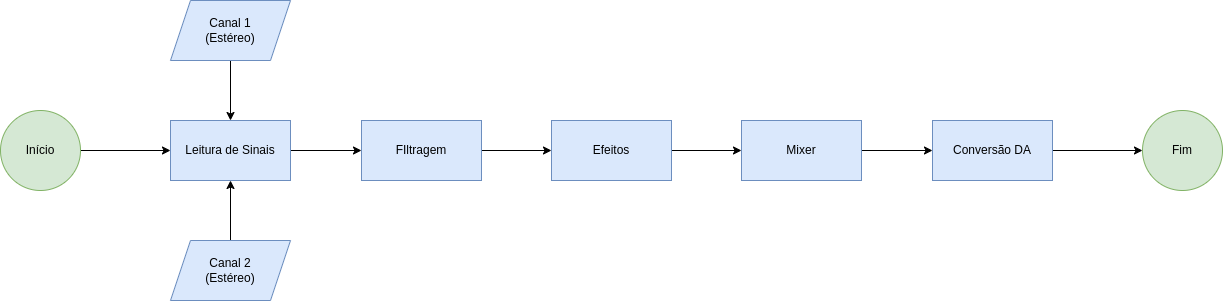
\includegraphics[width=\textwidth]{figuras/fig52.png}
    \caption{fluxograma geral do \textit{mixer}}
    \label{fig52}
\end{figure}

Os sinais provenientes de arquivos de música \textit{.wav} locais entram no sistema e são divididos em \textit{buffers}. Simultaneamente, é feita uma leitura dos valores atuais dos controles disponíveis na interface.

Com os valores dos parâmetros obtidos, a filtragem dos sinais e o processamento dos efeitos são realizados novamente para ajustar o comportamento dos sinais conforme os novos valores dos controles.

Finalmente, os sinais filtrados e os efeitos são combinados e convertidos para o formato analógico, para que possam ser reproduzidos.

Nas subseções abaixo, cada bloco presente no fluxograma geral do sistema (Figura \ref{fig52}) será detalhado em seus aspectos conceituais e processuais por meio de um subfluxograma, que descreve o processamento interno.

\subsection{Bloco de Leitura de Sinais}

Os sinais lidos incluem os sinais provenientes de arquivos digitais e os de controle provenientes de dois potenciômetros e um botão de duas posições. Os potenciômetros são utilizados para ajustar a frequência central e a quantidade de efeito desejado, enquanto o botão de duas posições é utilizado para selecionar o efeito desejado.

\begin{figure}[h]
    \centering
    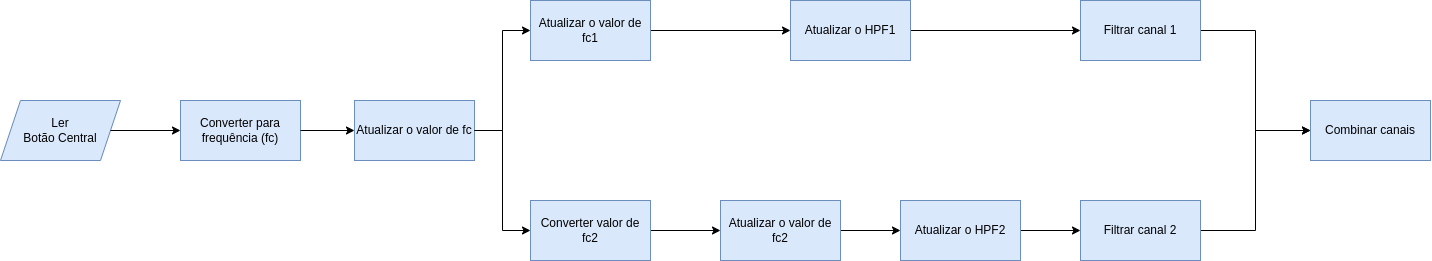
\includegraphics[width=\textwidth]{figuras/fig54.png}
    \caption{bloco de leitura de sinais}
    \label{fig54}
\end{figure}

Assim, conforme a Figura \ref{fig54}, todos os sinais analógicos de controle passarão por uma conversão analógico-digital, para que, em seguida, algumas variáveis tenham seus valores atualizados. Enquanto isso, os sinais de música obtidos de arquivos digitais já se encontram em formato digital, mas são transformados em sequência de \textit{buffers}.

\subsection{Bloco de Filtragem}

No bloco de filtragem, os sinais já estão no domínio digital. Primeiramente, deve-se ler a posição do botão central, que é obtida a partir da conversão de um sinal analógico proveniente de um potenciômetro, convertido de um sinal elétrico para um sinal digital.

Com a posição do botão, que estará em um intervalo de valores quantizados, realiza-se a normalização e conversão para um valor de frequência de corte, variando entre 20 e 22.050 Hz.

Este valor de frequência de corte é utilizado para atualizar o filtro passa-altas do canal 1, que então realiza a filtragem do sinal correspondente.

Para o canal 2, um novo valor de frequência de corte é calculado usando a expressão da Equação \ref{eq:05}. O filtro passa-altas deste canal é então ajustado conforme a nova frequência de corte, conforme ilustrado na Figura \ref{fig55}.

No bloco de filtragem, todos os sinais analógicos já estão codificados de forma que podem ser processados digitalmente. A frequência de corte central (\textit{fc}) varia entre 20 e 22.050 Hz, e os valores são atribuídos aos parâmetros \textit{fc$_{1}$} e \textit{fc$_{2}$}.

\begin{figure}[h]
    \centering
    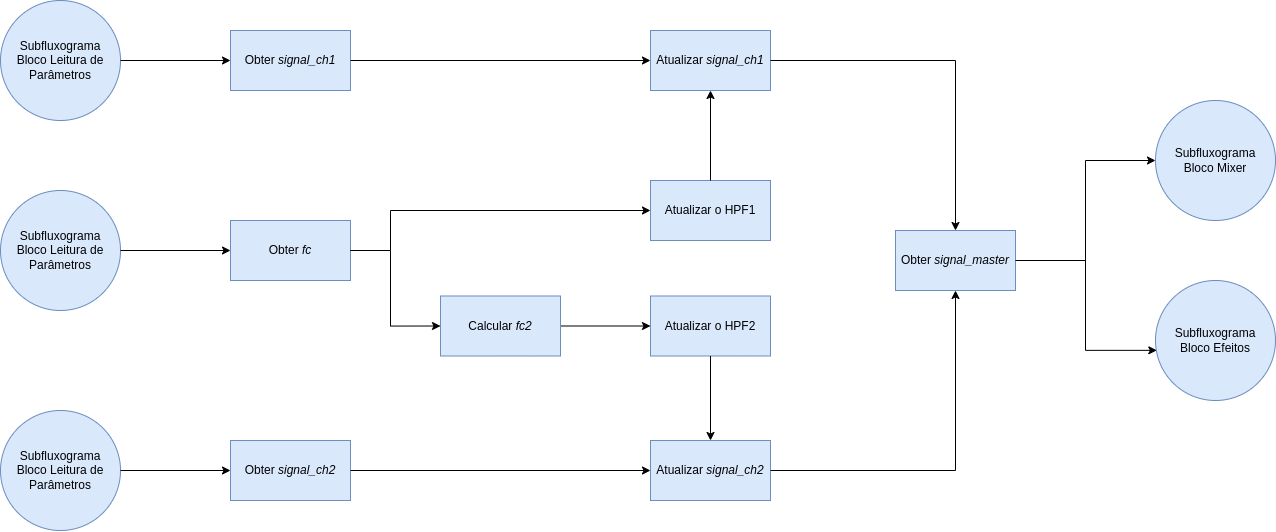
\includegraphics[width=\textwidth]{figuras/fig55.png}
    \caption{bloco de filtragem}
    \label{fig55}
\end{figure}

No subfluxograma da Figura \ref{fig55}, \textit{fc} representa a frequência de corte central, lida e convertida a partir do botão central; \textit{fc$_{1}$} é a frequência de corte para o filtro passa-altas 1 (HPF1) e \textit{fc$_{2}$} é a frequência de corte para o filtro passa-altas 2 (HPF2).

Ao final deste processo, os sinais dos dois canais são combinados, resultando no sinal \textit{signal\_master}, que é enviado ao bloco de processamento de efeitos.

\subsection{Bloco de Efeitos}

Os efeitos do \textit{mixer} podem ter seus parâmetros de reverberação e atraso configurados conforme o botão de quantidade de efeito. O parâmetro de reverberação é ajustado para 1 segundo, e o intervalo de atraso (em milissegundos) é configurado de acordo com a quantidade de efeito desejado.

\begin{figure}[h]
    \centering
    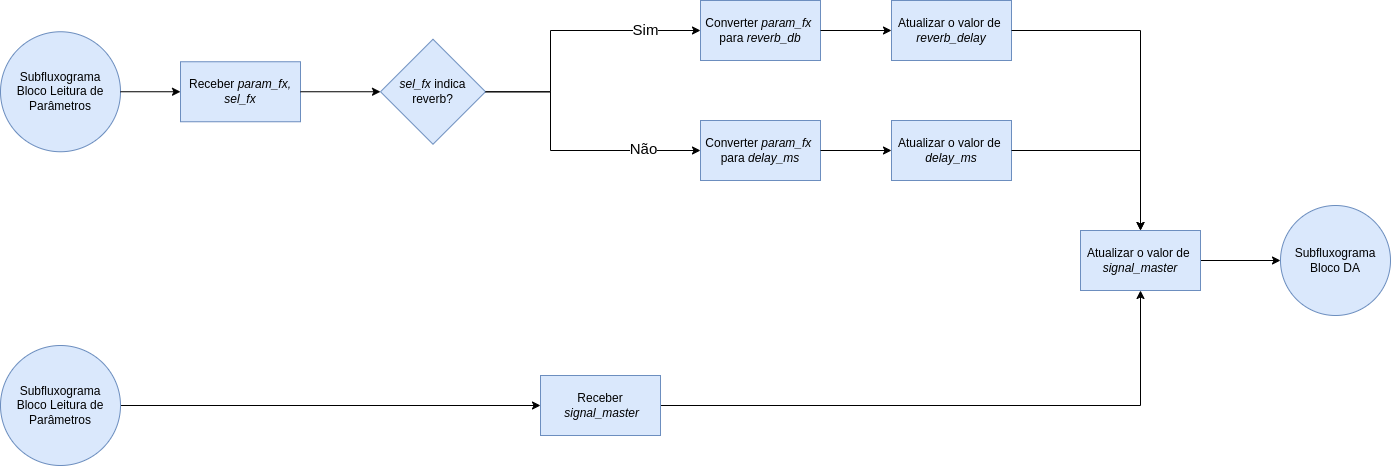
\includegraphics[width=\textwidth]{figuras/fig56.png}
    \caption{bloco de efeitos}
    \label{fig56}
\end{figure}

Além disso, o usuário pode selecionar qual efeito deseja utilizar através de um botão de duas posições, conforme ilustrado na Figura \ref{fig56}. Os parâmetros de seleção e quantidade de efeitos são obtidos do bloco de leitura de sinais. Ao final deste bloco, o sinal filtrado, já com o efeito aplicado, é atribuído ao \textit{signal\_master}.

\subsection{Bloco de Conversão DA}

O sinal de saída obtido pelo bloco \textit{Efeito} precisa ser convertido de digital para analógico para que possa ser reproduzido em um sistema de som.

\begin{figure}[h]
    \centering
    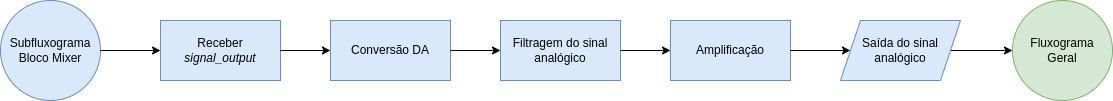
\includegraphics[width=\textwidth]{figuras/fig59.png}
    \caption{bloco de conversão digital-analógico}
    \label{fig59}
\end{figure}

Conforme mostrado na Figura \ref{fig59}, o sinal digital passará por um processo de conversão digital-analógico, para que possa ser finalmente reproduzido por caixas de som.

\newpage
\section{Prova de Conceito}

Nesta seção, é apresentada uma implementação em um ambiente virtual que simula a lógica de funcionamento do sistema.

\subsection{\textit{PureData}}

O \textit{PureData} \cite{puredata} é um ambiente de música computacional programável, projetado para análise, síntese e processamento de áudio em tempo real através de sinais digitais.

Esse ambiente permite a criação de sistemas de processamento de áudio utilizando blocos programáveis, com funções implementadas tanto pelos seus criadores quanto pela extensa comunidade de usuários.

\begin{figure}[h]
    \centering
    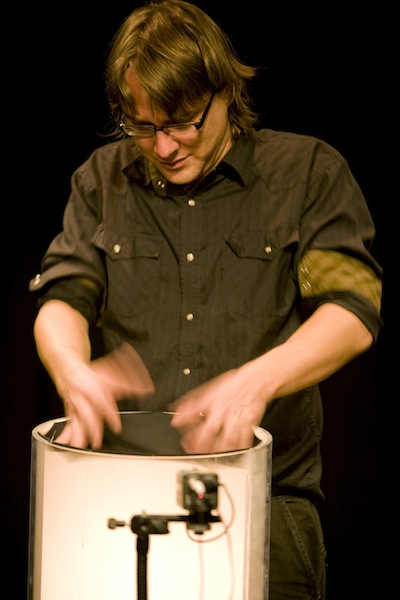
\includegraphics[width=0.3\textwidth]{figuras/fig79.jpg}
    \caption{Silent Drum de Jaime Oliver}
    \label{fig78}
\end{figure}

O \textit{PureData} contém uma extensa comunidade que desenvolve diversos tipos de projetos como instalações de arte interativas, geradores de música ambientes totalmente automatizados, uma bateria que utiliza visão computacional para controle da música, como se encontra na Figura \ref{fig78}, emuladores de equipamentos musicais, 
Outras aplicações incluem gravação, processamento e edição de áudio, \textit{samplers} e instalações de arte interativas que podem integrar sensores ou sistemas de áudio multicanal, além de projetos de projeção mapeada e muitos outros.

No \textit{PureData}, foi possível desenvolver uma prova de conceito que abrange a lógica do botão central para controle das frequências de corte, bem como o funcionamento dos efeitos. Para simular os sinais de entrada, foram utilizados arquivos \textit{.wav} locais.

A demonstração do sistema se divide em duas principais funcionalidades: filtragem e efeitos.

\subsection{Implementação de Filtragem}

A filtragem é realizada lendo dois arquivos de música no formato WAV, utilizando as funções \texttt{open}, \texttt{start} e \texttt{stop} para localizar, iniciar e parar a reprodução, respectivamente. Em seguida, o comando \texttt{readsf\textasciitilde\ 2 1e+06} é utilizado para configurar a leitura dos sinais em estéreo com um milhão de amostras no \textit{buffer}. Este processo é repetido para ambos os arquivos.

Para aplicar a filtragem, utiliza-se a função \texttt{hip\textasciitilde}, que implementa um filtro passa-altas. No entanto, o argumento da função varia entre o canal 1 e o canal 2. Como mostrado na Figura \ref{fig24}, o canal 1 ("FC do HPF1") recebe diretamente o parâmetro \textit{fc}, proveniente do \textit{slider} azul.

Por outro lado, o filtro passa-altas do canal 2 ("FC do HPF2") utiliza um valor ajustado por uma expressão anterior, conforme a Equação \ref{eq:05}. Esse ajuste assegura que uma pequena variação em \textit{fc$_{1}$} resulte em uma grande variação em \textit{fc$_{2}$}, e vice-versa. Além disso, em frequências centrais, a variação entre os canais torna-se mais semelhante. A Equação \ref{eq:05} descreve um círculo com raio igual à frequência de amostragem, com o botão centralizado no ponto (22050, 22050).

\begin{equation}  \label{eq:05}
    fc_2 = 22050 - \sqrt{22050^2 - (fc - 22050)^2}
\end{equation}

O ajuste na Equação \ref{eq:05} é projetado para ponderar mudanças nas frequências, pois mudanças lineares não são eficazes com um controle centralizado, como demonstrado pelas frequências dos canais na Figura \ref{fig45}.

\begin{figure}[h]
    \centering
    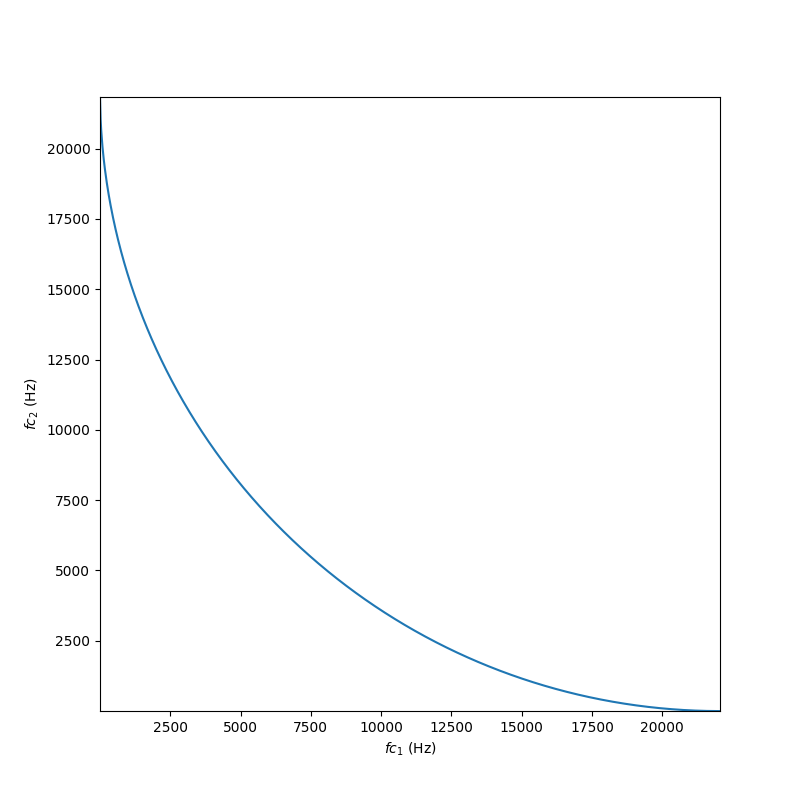
\includegraphics[width=0.7\textwidth]{figuras/fig45.png}
    \caption{expressão para a \textit{fc$_{2}$}}
    \label{fig45}
\end{figure}

Mudanças na ordem de centenas no canal 1 têm pouco impacto no canal 2, uma vez que as baixas frequências têm um ganho maior em relação às altas frequências. Essa lógica também se aplica ao outro extremo do controle de frequência.

\begin{figure}[h]
    \centering
    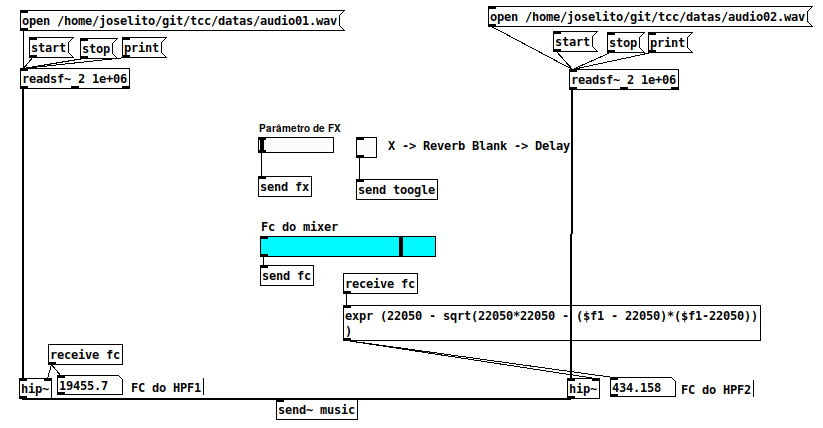
\includegraphics[width=0.9\textwidth]{figuras/fig44.png}
    \caption{lógica de funcionamento do botão central no \textit{PureData}}
    \label{fig44}
\end{figure}

Na Figura \ref{fig44}, a frequência obtida do botão central, denotada como \( f_c \), varia de 0.2 a 22050 Hz. A frequência de corte do canal 1, referida como FC do HPF1, é equivalente a \( f_c \). A frequência de corte do canal 2, identificada como FC do HPF2, é calculada pela Equação \ref{eq:05}. O sinal resultante, \texttt{send\textasciitilde\ music}, é a soma dos sinais filtrados dos canais 1 e 2.

\newpage
\subsection{Implementação de Efeitos}

A implementação dos efeitos utiliza três parâmetros principais: um botão \texttt{toggle} para alternar entre os efeitos \textit{delay} e \textit{reverb}; um \textit{slider} para ajustar parâmetros internos dos efeitos; e a frequência de corte do botão central, que automatiza o volume do efeito.

\begin{figure}[h]
    \centering
    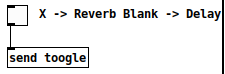
\includegraphics[width=0.3\textwidth]{figuras/fig46.png}
    \caption{botão de seleção de efeito no \textit{PureData}}
    \label{fig46}
\end{figure}

O botão \texttt{toggle} é usado para alternar entre os efeitos. Com duas posições disponíveis, sempre um efeito está ativo. Para mudar o efeito, basta alterar a posição do botão, conforme mostrado na Figura \ref{fig46}.

\begin{figure}[h]
    \centering
    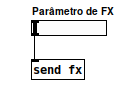
\includegraphics[width=0.2\textwidth]{figuras/fig47.png}
    \caption{botão de quantidade de efeito no \textit{PureData}}
    \label{fig47}
\end{figure}

O \textit{slider} é utilizado para ajustar os parâmetros internos de cada efeito. Seus valores variam de 0 a 1, e o botão está ilustrado na Figura \ref{fig47}.

Cada efeito utiliza o parâmetro \textit{fx} do \textit{slider} e o ajusta conforme necessário. No caso do \textit{reverb}, o valor de \textit{fx} é multiplicado por 100 para determinar a quantidade de \textit{dB} que permanece na música após 1s. Para o \textit{delay}, o valor é multiplicado por 1000, transformando-se no intervalo de tempo em \textit{ms} que o efeito permanecerá na música.

\begin{figure}[h]
    \centering
    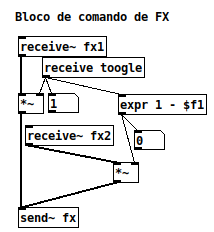
\includegraphics[width=0.3\textwidth]{figuras/fig48.png}
    \caption{lógica de seleção de efeito no \textit{PureData}}
    \label{fig48}
\end{figure}

A lógica de seleção do efeito é apresentada na Figura \ref{fig48}. Os comandos \texttt{receive\textasciitilde\ fx} inserem os efeitos como entrada. Cada volume do efeito é multiplicado pelo valor do \texttt{toggle}; um deles é multiplicado pelo valor atual enquanto o outro é multiplicado pelo inverso, permitindo que o botão \texttt{toggle} funcione como um alternador entre os efeitos.


\begin{figure}[h]
    \centering
    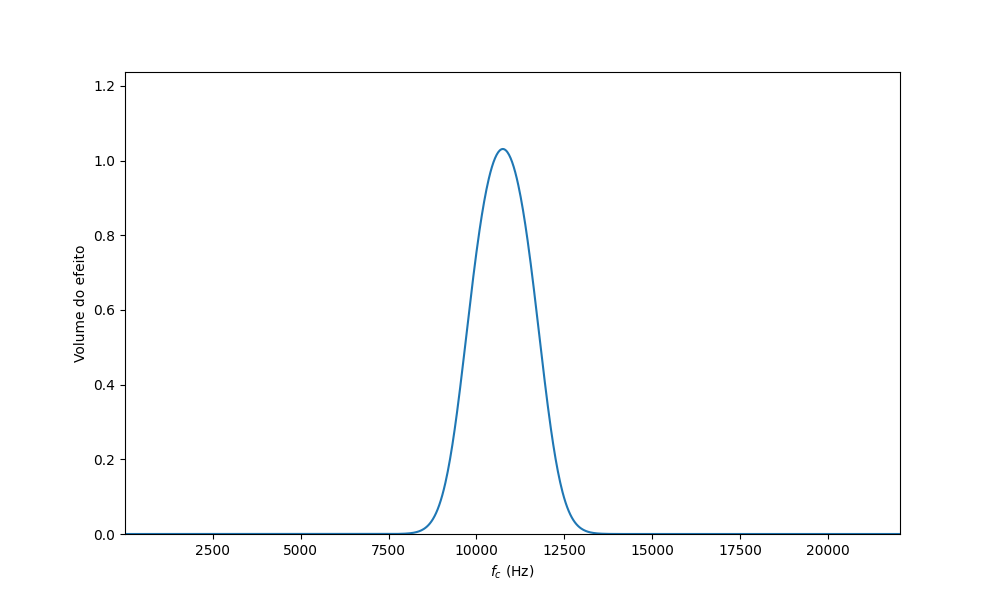
\includegraphics[width=0.9\textwidth]{figuras/fig49.png}
    \caption{variação do volume dos efeitos no \textit{PureData}}
    \label{fig49}
\end{figure}

No sistema, o volume do efeito é ajustado automaticamente com base na posição do botão central, ou seja, nas frequências de corte. A Figura \ref{fig49} ilustra a variação do volume dos efeitos em função da frequência central.

\begin{figure}[h]
    \centering
    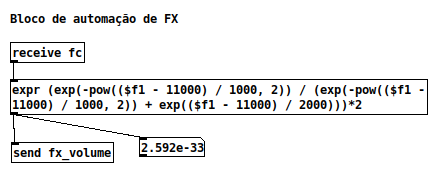
\includegraphics[width=0.6\textwidth]{figuras/fig50.png}
    \caption{implementação da variação do volume dos efeitos no \textit{PureData}}
    \label{fig50}
\end{figure}

\newpage
No \textit{PureData}, o bloco de automação do volume dos efeitos é implementado usando as operações mostradas na Figura \ref{fig50}.

\begin{figure}[h]
    \centering
    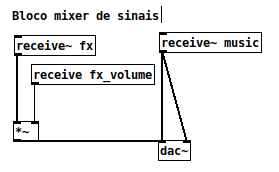
\includegraphics[width=0.3\textwidth]{figuras/fig51.png}
    \caption{soma dos sinais filtrados e dos efeitos no \textit{PureData}}
    \label{fig51}
\end{figure}

Finalmente, o sinal dos efeitos é multiplicado pelo volume dos efeitos e, em seguida, somado ao sinal filtrado, resultando no sinal de saída. Esse sinal é processado por um bloco de conversão digital-analógico e, por fim, é reproduzido. O bloco que realiza a soma dos sinais está representado na Figura \ref{fig51}.

\newpage
\section{Proposta de Implementação}

Em linhas gerais, a proposta de implementação desse projeto envolve a utilização de uma \textit{Raspberry Pi} para a escolha das músicas a serem enviadas ao \textit{mixer}, para a aquisição de sinais analógicos responsáveis pelos controles de frequência e efeitos, além de, através do conector de 3,5 mm da placa, realizar a ligação ao equipamento de sistema de som para a reprodução. 

\subsection{Implementação em Hardware}

Esta seção descreve a proposta de implementação em \textit{hardware} para o sistema de mixagem de áudio, abrangendo conectores, botões e outros componentes essenciais.

\subsubsection*{Botões}
A interação do usuário é crucial para ajustar parâmetros como frequência de corte, quantidade de efeitos e seleção do efeito desejado. Para isso, serão utilizados dois \textit{knobs} e uma chave.


\begin{figure}[h]
    \centering
    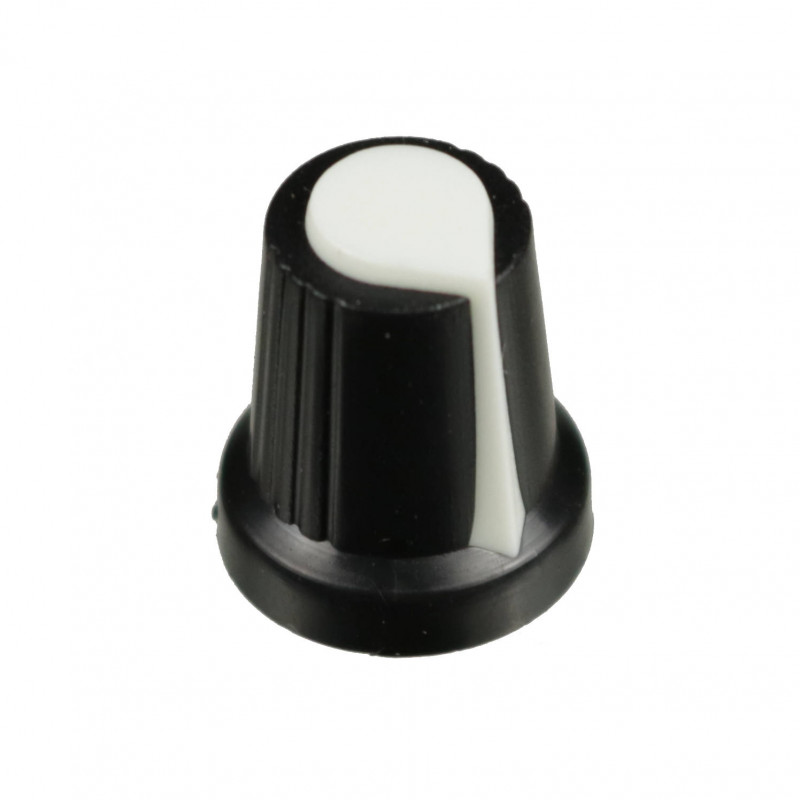
\includegraphics[width=0.3\textwidth]{figuras/fig61.jpg}
    \caption{botão \textit{knob} para frequência central e efeitos \cite{robocore}}
    \label{fig61}
\end{figure}

Os \textit{knobs} serão equipados com potenciômetros. Eles são alimentados por uma tensão, e sua posição é medida por uma tensão de saída proporcional à tensão de entrada. Essa configuração é preferida devido à precisão oferecida pelo ajuste com dois dedos, que proporciona uma mudança de frequência precisa. A Figura \ref{fig61} mostra um exemplo esperado de um \textit{knob} para ajustar a frequência central e de intensidade de efeitos.

\begin{figure}[h]
    \centering
    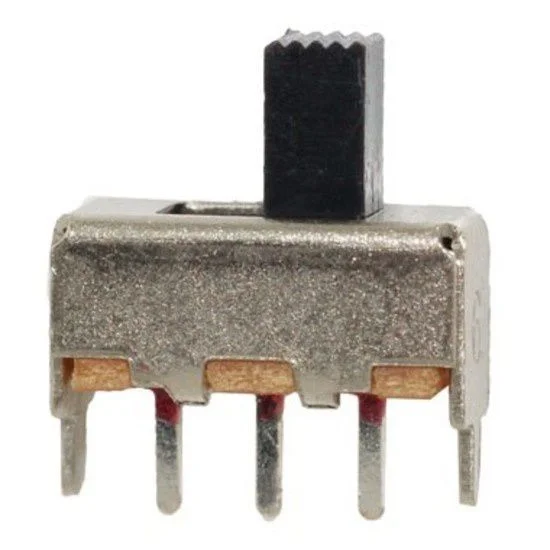
\includegraphics[width=0.3\textwidth]{figuras/fig62.png}
    \caption{botão para seleção do efeito \cite{evea}}
    \label{fig62}
\end{figure}

A chave será utilizada para selecionar entre dois efeitos distintos, gerando dois níveis de tensão: um nulo e outro de alimentação. Cada nível corresponderá a um efeito diferente. Um exemplo de botão para essa finalidade é mostrado na Figura \ref{fig62}.

Para ajustar a quantidade de efeitos desejada, será utilizado um botão semelhante ao \textit{slider}, com a mesma abordagem de controle e ajuste.

\paragraph*{Conversão AD}

A conversão analógica-digital será empregada na aquisição dos sinais de controle, ou seja, para dois potenciômetros, utilizando um conversor PCF8591, Figura \ref{fig64}, que conta com uma resolução de 8 \textit{bits}. 

\begin{figure}[h]
    \centering
    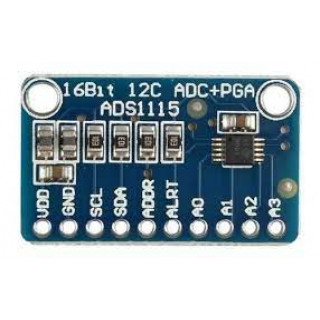
\includegraphics[width=0.5\textwidth]{figuras/fig64.jpg}
    \caption{PF8591 - conversor analógico-digital de 8 \textit{bits} \cite{saravaticomponentes}}
    \label{fig64}
\end{figure}

Para que esses sinais de controle sejam lidos, a comunicação I2C da \textit{Raspberry Pi} deve estar habilidada para a leitura.

\paragraph*{Raspberry Pi}

A unidade de processamento é o dispositivo responsável pela realização do processamento dos sinais. 

\begin{figure}[h]
    \centering
    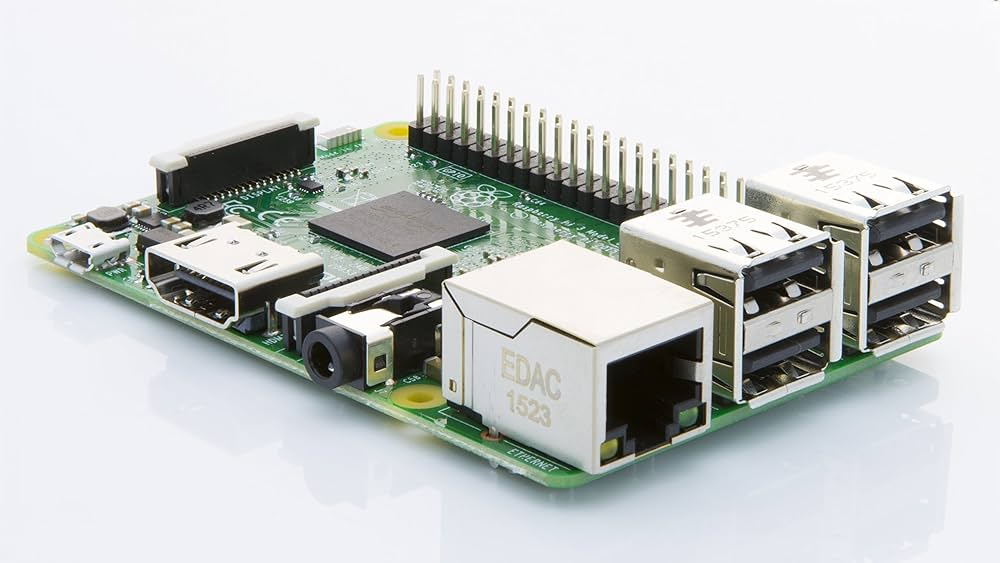
\includegraphics[width=0.5\textwidth]{figuras/fig65.jpg}
    \caption{\textit{Raspberry Pi} para processamento dos sinais \cite{adrenalineDisplaysLanar}}
    \label{fig65}
\end{figure}

Para essa tarefa, será utilizada uma \textit{Raspberry Pi}, que oferece um bom poder de processamento e flexibilidade em termos de linguagens de programação suportadas. A \textit{Raspberry Pi} é mostrada na Figura \ref{fig65}.

\paragraph*{Conversão DA}

A conversão digital-analógico é necessária para que o sinal final, após o processamento, possa ser reproduzido por sistemas de áudio que utilizam sinais analógicos. A \textit{Raspberry Pi} possui uma saída/entrada de áudio com conector de 3.5mm, conforme ilustrado na Figura \ref{fig20}.

\paragraph*{Diagrama de Conexões}

O diagrama de pinagem, Figura \ref{fig80},  contém o conversor AD e a \textit{Raspberry Pi 4 B}, e compreende as conexões necessárias para que os sinais de controle sejam lidos pelo conversor PCF8591 e transferidos via I2C para a \textit{Raspberry}.

\begin{figure}[h]
    \centering
    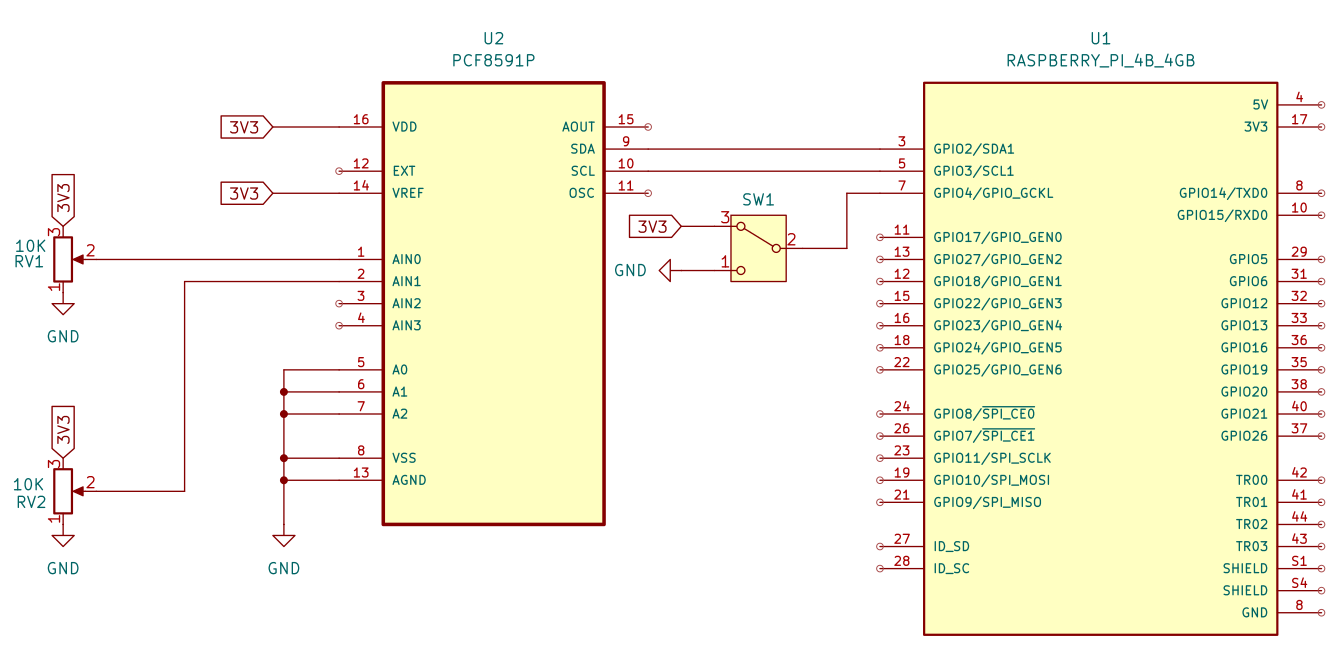
\includegraphics[width=1\textwidth]{figuras/fig80.png}
    \caption{Diagrama de Conexões}
    \label{fig80}
\end{figure}

No circuito integrado PCF8591, as entradas A0, A1 e A2 correspondem à configuração do endereço I2C, necessário para que a \textit{Raspberry} consiga identificar o dispositivo e receber as leituras realizadas. Naturalmente, esse dispositivo possui endereço \textit{0x48}. Porém, quando os pinos A0, A1 e A2 estavam abertos, havia uma flutuação do endereço. Para estabilizar o endereço, foi necessário o aterramento dessas entradas de endereço. 

Além disso, as entradas utilizadas para as leituras dos \textit{knobs} seletor de frequência de corte (AIN0) e da intensidade do efeito (AIN1), utilizou-se as duas primeiras entradas. Para que se obtenha as leituras específicas dessa entrada, no código de aquisição de sinal, selecionou-se as entradas \textit{0x40} e \textit{0x41}, correspondentes respectivamente às entradas \textit{AIN0} e \textit{AIN1}.

Outro componente utilziado foi a chave de duas posições, no diagrama \ref{fig80}, denominado de \textit{SW1}. Essa chave é capaz de mandar ao GPIO da \textit{Raspberry} o nível lógico alto (3V3) ou baixo (GND). Com esses níveis, é possível descobrir se o usuário deseja que o efeito 1 ou o 2 seja executado naquele momento.

Para a reprodução do sinal de saída, utilizou-se a entrada de 3,5 m nativa da \textit{Raspberry}.

\paragraph*{Lista de Materiais}

Para a implementação desse projeto, fez-se necessária a utilização dos componentes abaixo:

\begin{itemize}[left=0pt, label=$\bullet$, itemsep=5pt] % Customize a lista
    \item 1 Raspberry Pi
    \item 1 CI conversor AD/DA PCF8591
    \item 2 potenciômetros de 10 k$\Omega$
    \item 1 chave HH de 2 posições
    \item 1 cabo 3,5 mm
    \item 1 fonte 5 VDC com cabo USB-C
    \item 1 computador para acesso remoto
\end{itemize}

Para realizar a alimentação da \textit{Raspberry}, faz-se necessária a fonte com um cabo USB-C. 


\subsection{Implementação em Software}

Para a implementação do processamento de sinais de áudio, o código foi estruturado em várias bibliotecas, cada uma contendo funções específicas para cada etapa do processamento. O fluxo começa com a declaração das variáveis necessárias para iniciar a aquisição dos sinais. Em seguida, os arquivos de áudio no formato \textit{.wav} são lidos e processados utilizando uma lógica de \textit{buffers}, que segmenta os dados para permitir um processamento contínuo e eficiente.

Com os segmentos de dados em mãos, diferentes processamentos são realizados, como filtragem e aplicação de efeitos. Após o processamento, os sinais são então reproduzidos.

[INSERIR UM DIAGRAMA DE ESTADOS PARA ESSA APLICAÇÃO]

Além disso, de forma cíclica, são realizadas aquisições de sinais de controle que permitem ajustar, em tempo real, parâmetros como a frequência de corte, a seleção dos efeitos e a intensidade aplicada.

\paragraph*{Definição e Alocação Inicial de Buffers}

No início da função principal, \verb|int main() {}|, são declarados ponteiros que terão papel fundamental ao longo do processamento de áudio. Esses ponteiros, \verb|*sinal1| e \verb|*sinal2|, irão armazenar os sinais de áudio completos, um para cada canal de áudio. Além disso, são definidos ponteiros para buffers, \verb|**buffers_sinal1| e \verb|**buffers_sinal2|, que serão usados para armazenar segmentos do sinal durante o processamento.

O tamanho do \textit{buffer} é definido pela variável \verb|buffer_size|, que pode ser ajustada de acordo com a necessidade da aplicação. No exemplo, o tamanho padrão do \textit{buffer} foi definido como 1024 amostras, o que permitirá um processamento em blocos de dados, facilitando a aplicação de filtros e efeitos. A quantidade total de \textit{buffers} a ser utilizada durante a execução será determinada posteriormente com base no tamanho total dos sinais de áudio.

Este trecho inicial de código configura as variáveis básicas necessárias para garantir que o processamento ocorra em partes menores (segmentos), o que é essencial para operações eficientes em tempo real.

\paragraph*{Aquisição de Sinais de Áudio}

Para iniciar o processamento, a aquisição dos sinais é realizada por meio da leitura de arquivos \textit{.wav} locais, sendo que duas funções principais são responsáveis por essa tarefa: \verb|ler_wav_estereo| e \verb|ler_dois_wav_estereo|.

A função \verb|int ler_wav_estereo()| armazena os dados do arquivo \textit{WAV} em um \textit{buffer}. O arquivo de áudio é aberto e, caso ocorra algum erro, uma mensagem é exibida. Após a abertura do arquivo, seu cabeçalho é analisado para obter informações essenciais como número de canais, taxa de amostragem, \textit{bits} por amostra e tamanho total. Com esses dados, a memória é alocada para armazenar os sinais, que são então lidos e salvos.

Já a função \verb|ler_dois_wav_estereo()| faz uso de \verb|ler_wav_estereo()| para ler os dois arquivos a partir dos caminhos definidos. Ao invocar \verb|ler_wav_estereo()|, os sinais são alocados em \textit{arrays}.



\paragraph*{Geração dos Buffers}

O processamento de áudio realizado por esta aplicação é dinâmico, pois se adapta às novas variáveis de controle, como frequência de corte, escolha e intensidade de efeitos. Para garantir um processamento contínuo e eficiente, foi utilizada a função \linebreak \verb|gerar_buffers_circulares|, que cria \textit{buffers} de tamanho regular, os quais são utilizados como entradas para as funções de processamento. A função \verb|gerar_buffers_circulares| é responsável por gerar os \textit{buffers} circulares a partir dos sinais de áudio, alocando as memórias necessárias para armazená-los e preenchendo-os de forma a permitir o processamento contínuo dos sinais.

Antes de iniciar processamento, a função \verb|gerar_buffers_circulares| gera os \textit{buffers} circulares a partir dos dois sinais de áudio (\verb|sinal1| e \verb|sinal2|), alocando as memórias necessárias para armazená-los. Em vez de utilizar \textit{buffers} clássicos, a função adota o conceito de \textit{buffer} circular, permitindo que, ao atingir o final de um \textit{buffer}, o processamento continue a partir do início, assegurando um fluxo contínuo dos sinais. Primeiramente, a função calcula o número de \textit{buffers} necessários com base no tamanho total dos sinais e no tamanho de cada \textit{buffer}. Em seguida, ela aloca memória para os ponteiros que armazenarão os \textit{buffers} e, dentro de um laço, aloca memória para cada \textit{buffer} individualmente. Após garantir a alocação bem-sucedida, a função preenche os \textit{buffers} com os sinais, utilizando acesso circular para garantir que, ao atingir o final do sinal, os dados continuem sendo lidos a partir do início. Se algum erro ocorrer durante a alocação, a função retorna -1 após imprimir uma mensagem de erro; caso contrário, ela retorna 0, indicando que os \textit{buffers} foram criados e preenchidos com sucesso.

\paragraph*{Aquisição dos Parâmetros de Controle}

1) Explicar onde esses parâmetros são utilizados
2) Explicar quais componentes realizam essa aquisição
3) Explicar Qual a resolução desses sinais
4) Explicar com qual frequência ele é atualizados
5) Explicar como se obtém a frequência
5) Explicar o código que realiza essa aquisição e atribuição

\paragraph*{Conversão de Frequências de Corte}

1) Explicar como a frequência 2 é obtida

\paragraph*{Parâmetros do Filtro FIR}

A obtenção de um filtro tradicionalmente parte de especificações como banda de transição desejada em determinada frequência de corte, atenuações na banda rejeitada, erros e outros parâmetros. Porém, para a obtenção do filtro para essa aplicação, utilizou-se um método empírico. Esse método consistiu na obtenção da concentração de potência em uma música de referência antes e depois de uma filtragem, realizada no \textit{PureData}. 

Através de um código em \textit{Python}, aplicou-se uma DFT para se obter a contribuição, em relação à potência, da faixa entre 20 e 300 Hz. Em seguida, uma filtragem padrão do \textit{software} foi realizada e novamente se obteve a concentração de potência dessa faixa. Com as duas concentrações, antes e depois da filtragem, obteve-se um parâmetro para realizar uma iteração para elencar a ordem necessária para que a rejeição da banda obtivesse o mesmo comportamento.

Assim, utilizando outro código em \textit{Python}, implementou-se um filtro que retornasse essa concentração após a filtragem. O código iterou a ordem do filtro até que se obtivesse uma atenuação maior que a obtida pelo \textit{PureData} e se chegou a ordem 121. 

A seguir, foi necessário descobrir qual janelamento produziria esse desempenho de atenuação através de um teste que retornou a concentração de potência na banda rejeitada com ordem 121 em 11 tipos de janelas. O janelamento que obteve melhor resultado foi o \textit{Hamming}. Dessa forma, o filtro para a aplicação foi obtido. 

\paragraph*{Matriz de Coeficientes do Filtro FIR}

Quando o valor analógico do potenciômetro é quantizado, obteve-se 256 níveis de quantizações já que o conversor analógico digital escolhido possui resolução de 8 \textit{bits}. Dessa forma, o código possui 256 frequências possíveis para realizar o processamento, ou seja, 256 combinações possíveis de coeficientes para o filtro. Dessa forma, antes de se realizar o processamento, esses coeficientes são calculados e alocados em um vetor, para que, conforme novas frequências de corte sejam obtidas, utiliza-se os coeficientes já criados e alocados nesse vetor, ao invés de realizar o cálculo novamente. Essa solução foi aplicada para evitar o cálculo dos coeficientes a cada ciclo.

A função \verb|generate_hamming_highpass_filter()| realiza duas etapas principais para gerar os coeficientes do filtro passa-altas, pois utiliza o método de janelamento para projeto de filtro FIR, ou seja, obtém-se o filtro ideal para determinada frequência de corte, e em seguida, obtém-se os coeficientes para a janela escolhida, conforme a ordem determinada. De forma mais detalhada, primeiramente, calcula-se a resposta ideal do filtro utilizando a função \textit{sinc}. A resposta ideal é obtida na frequência de corte normalizada em função da frequência de \textit{Nyquist}; e os coeficientes são obtidos para permitir a passagem das altas frequências enquanto atenuam as baixas. Aplica-se a janela de \textit{Hamming} para suavizar a resposta do filtro ideal e minimizar o efeito \textit{Gibbs} nos extremos do filtro, melhorando sua resposta em frequência.

A matriz resultante contém os coeficientes dos filtros para todas possíveis frequências de corte, cuja quantidade é limitada pela quantização dos valores analógicos no vetor \verb|frequencias_log[]|.

\paragraph*{Aplicação do Filtro FIR}

A função \verb|aplicar_filtro_FIR_buffer| aplica o filtro FIR a um sinal armazenado em um \textit{buffer} circular. O objetivo da função é percorrer cada amostra do sinal e aplicar os coeficientes do filtro FIR. A função recebe como parâmetros o \verb|buffer_sinal|, que é o sinal de entrada, o \verb|buffer_sinal_filtrado|, que armazenará o sinal após a filtragem, o \verb|buffer_size|, que indica o tamanho do \textit{buffer}, os \verb|coeficientes|, que contém os coeficientes do filtro FIR, e a \verb|ordem|, que define o número de coeficientes a serem usados no cálculo da soma ponderada.

Após processar todas as amostras anteriores, a função limita o valor do \verb|acumulador| para garantir que o valor filtrado não ultrapasse os limites de 16 bits, ajustando-o para o valor máximo (\verb|MAX_16BIT|) ou mínimo (\verb|-MAX_16BIT|) permitido. Essa etapa é importante para evitar distorções causadas por estouros de valores. Finalmente, o valor filtrado é armazenado no \verb|buffer_sinal_filtrado[j]|, que contém o sinal de saída filtrado.

O processo de aplicar os coeficientes do filtro FIR a cada amostra do sinal, através da soma ponderada das amostras anteriores, é o mecanismo gerado a partir de um comportamento do sinal no domínio da frequência, a partir da frequência de corte e da ordem do filtro, que modificam os sinais no domínio do tempo, permitindo que a operação de rejeição de determinada banda seja efetiva nos sinais representados no tempo. E é dessa forma que se pode sentir, ao escutar o som filtrado, que determinados elementos foram excluídos dos sinais.

\paragraph*{Efeito - Delay}

Para o processamento do \textit{delay} no sinal de áudio, implementou-se uma biblioteca denominada \verb|delay.h|, que contém duas funções: \verb|aplicar_delay()|, responsável por aplicar o efeito nos \textit{buffers} e \verb|liberar_delay()|, responsável por limpar os \textit{buffers} após a utilização dos \textit{buffers} processados. 

O arquivo \verb|delay.c| declara globalmente um ponteiro para o \textit{buffer} circular onde as amostras são armazenadas, bem como uma variável para a localização dentro do \textit{buffer}. Os parâmetros para essa função são \verb|float *buffer|, \verb|int buffer_size|, \verb|float wetness| e \verb|float feedback|, sendo respectivamente, o ponteiro para o \textit{buffer} que contém as amostras a serem processadas, o tamanho do \textit{buffer} de áudio utilizado, o parâmetro que determina a composição do sinal final entre o sinal filtrado e o sinal com efeito e a quantidade de realimentação do sinal atrasado.

A função começa definindo o valor do delay: o delay é inicialmente definido como 500 milissegundos e depois convertido para amostras (\textit{delay\_samples}), com base na taxa de amostragem. Se esse valor exceder o máximo permitido (\textit{MAX\_DELAY\_SAMPLES}), ele é limitado. 

Para cada amostra no buffer de áudio, a função obtém a amostra atrasada do \textit{delay\_buffer} com base na posição atual. Em seguida, a nova amostra é uma mistura do sinal original (\textit{buffer[i]}) com o sinal atrasado, controlada pelo parâmetro \textit{wetness}. O sinal atrasado também recebe uma realimentação proporcional ao parâmetro \textit{feedback}, o que faz com que ele seja repetido várias vezes, criando um efeito de eco contínuo. 

O \textit{delay\_buffer} é atualizado com a nova amostra somada ao sinal de feedback. A posição do \textit{delay\_buffer} é incrementada ciclicamente, reiniciando quando atinge o tamanho máximo de delay (\textit{delay\_samples}). Finalmente, a amostra processada é armazenada no \textit{buffer[i]}, substituindo o valor original.

\paragraph*{Efeito - Reverb}

O efeito \textit{reverb} utiliza o conceito presente no efeito \textit{delay} para ser implementado, com a diferença de que neste efeito, uma série de ecos são aplicados tão rapidamente e de forma difusa que se cria uma sensação de espacialidade ao som. Portanto, os ecos do \textit{reverb} são muito mais curtos e mais numerosos em relação ao \textit{delay}, para que se dê uma sensação de profundidade, como se o som estivesse sendo aplicado a um ambiente real.

Para a implementação desse efeito tão usual na mixagem de \textit{Djs}, defini-se os seguintes parâmetros: \verb|buffer_size|, que dita a quantidade de amostras em um \textit{buffer}, \verb|sample_rate|, que é a frequência de amostragem do sinal corrente, e \verb|maxDelay|, que é o máximo atraso a ser utilizado no \textit{delay}, que nesse caso foi 0.5 segundos, devido a um cálculo realizado de tempo por batida na música, levando em consideração 125 BPM.

O processo de aplicação do efeito \textit{reverb} se inicia com a alocação de um \textit{buffer} para armazenar o atraso de cada amostra, levando em conta o parâmetro de atraso máximo.

Em seguida, utilizando o tamanho padrão do \textit{buffer}, aplica-se o efeito de \textit{reverb}, ou seja, o sinal atrasado do \textit{delay} é recuperado em sinais posteriores, de forma que o parâmetro \textit{wetness} indica a presença do efeito e do sinal original; quanto maior o \textit{wetness}, mais a amostra com efeitos é aplicada ao sinal de saída. A reintrodução de amostras anteriores é controlada pelo parâmetro \textit{feedback}, enquanto o peso para o sinal sem efeito e o com efeito é regulado pelo parâmetro \textit{wetness}. Dessa forma, é realizado o efeito \textit{reverb} nesse caso, por um banco de atrasos.

Portanto, o processamento desse efeito ocorre amostra por amostra presente no buffer utilizando as seguintes etapas:

O \textit{loop} \verb|for (int i = 0; i < numSamples; i++)| percorre cada amostra do sinal de áudio (\textit{buffer}), processando uma amostra de cada vez.


A variável \verb|drySignal| armazena o valor da amostra original (não processada), extraída do \verb|buffer[i]|.

A variável \verb|wetSignal| é preenchida com o valor da amostra do \textit{buffer} de \textit{delay} na posição atual \verb|delayIndex| (\textit{buffer} esse que é iniciado com zeros, mas que ao longo dos ciclos, funciona como a memória do efeito). Esse valor representa o sinal com o efeito de \textit{reverb} aplicado (atraso e \textit{feedback}).

A fórmula \sloppy
\texttt{buffer[i] = (1.0f - wetness) * drySignal + wetness * wetSignal} calcula a mistura entre o sinal original (seco) e o sinal processado (molhado), com base no valor de \verb|wetness|. Quanto maior o valor de \verb|wetness|, maior será a contribuição do sinal com \textit{reverb} no resultado final.

A variável \verb|feedbackSignal| é calculada como \verb|wetSignal * feedback|, que determina a quantidade de \textit{feedback} a ser aplicada ao \textit{buffer} de \textit{delay}. O valor de \verb|feedback| controla a intensidade do efeito de \textit{reverb} (quanto maior o \textit{feedback}, mais ecos serão gerados).

O \textit{buffer} de \textit{delay} \verb|delayBuffer[delayIndex]| é atualizado com o valor do sinal seco (\verb|drySignal|) somado ao \verb|feedbackSignal|. Isso garante que a amostra processada seja armazenada no \textit{buffer} de \textit{delay} para ser reutilizada em iterações futuras, criando o efeito de eco do \textit{reverb}.

O índice \verb|delayIndex| é incrementado e ajustado para garantir que ele seja cíclico. O cálculo \verb|(delayIndex + 1) % maxDelay| faz com que o índice retorne ao início do \textit{buffer} quando atingir o limite máximo (\verb|maxDelay|), mantendo o processamento contínuo das amostras.

Em resumo, o código processa cada amostra do áudio, aplica a mistura do sinal original com o sinal atrasado (com o efeito de \textit{reverb}), aplica \textit{feedback} para intensificar os ecos, e atualiza o \textit{buffer} de \textit{delay} de forma cíclica para criar o efeito de \textit{reverb} contínuo.


\paragraph*{Reprodução dos Buffers}

A reprodução das amostras é acionada a cada final de ciclo de processamento dos \textit{buffers}. Para tal tarefa, utilizou-se uma biblioteca de áudio chamada \textit{PortAudio} para implementar duas funções que cobrem as seguintes tarefas: inicialização do \textit{PortAudio} e a reprodução do \textit{buffer}.

A função \verb|inicializar_audio()| tem como objetivo inicializar o sistema de áudio, configurar o fluxo de saída de áudio e prepará-lo para a reprodução. Essas etapas foram implementadas, primeiramente, declarando uma variável global \verb|PaStream *stream|, e em seguida, com a inicialização do sistema de áudio através da função \verb|Pa_Initialize()|. Após a inicialização, configura-se o fluxo de dados com parâmetros como quantidade de canais de saída, tipo de dados, taxa de amostragem e tamanho do bloco, através da função \verb|Pa_OpenDefaultStream()|. Por fim, com o sistema de áudio e o fluxo inicializados e configurados, inicia-se a transmissão com a função \verb|Pa_StartStream()|. Portanto, a execução da função \verb|inicializar_audio()| é realizada apenas uma vez. 

A função que realizará propriamente a reprodução do áudio é a \verb|reproduzir_buffer()|, de modo que envia um \textit{buffer} para o dispositivo de saída de áudio, previamente configurado. Para realizar essa funcionalidade, a função \verb|Pa_WriteStream()| é invocada junto com os seguintes parâmetros: \verb|stream|, variável global, \verb|media_buffer|, amostras processadas após a aplicação dos efeitos, e \textit{buffer\_size}, o tamanho do \textit{buffer}. Dessa forma, \verb|reproduzir_buffer()| é invocada de forma recursiva, a cada final de ciclo de processamento de um \textit{buffer}.

\paragraph*{Processamento dos Buffers}

Com as funções que realizam cada etapa do processamento definidas e com suas entradas e saídas alinhadas, há uma função que reune a chamada dessas funções anteriores para cada \textit{buffer} denominada de \verb|int processar_buffers_circulares|.


Em seguida, inicia-se uma sequência de declarações e alocações de vetores e \textit{buffers} que serão consultados ou manipulados ao longo do processamento contínuo. Primeiramente, declara-se dois vetores essenciais para o processo de filtragem sendo um responsável pelas frequências de corte possíveis e outro pelos coeficientes do filtro FIR. Com os vetores declarados, chama-se as funções \verb|gerar_pontos_logaritmicos()| e \verb|gerar_matriz_coeficientes()|, que utilizarão esses vetores para alocar as frequências de corte e todos os conjuntos possíveis de coeficientes para essa aplicação. 

Alocações de espaço para os ponteiros dos \textit{buffers}, que serão utilizados para os sinais filtrados, são realizadas utilizando a função \verb|malloc()|, de forma que ambos canais estão contemplados por esses ponteiros. Na sequência, os \textit{buffers} em si são alocados de forma iterativa até que se crie espaços para o número total de \textit{buffers} definidos pela duração das músicas. Para as duas etapas de alocações, são realizados testes que verificam o êxito da criação e apontamento das memórias solicitadas.

Subsequentemente, inicia-se propriamente o processo contínuo de processamento dos sinais. Adquiri-se os parâmetros de controle (frequência de corte, seleção e intensidade do efeito) que serão usados nas funções específicas de cada etapa, e os coeficientes do filtro FIR são escolhidos em função da frequência de corte e alocados em um vetor denominado \verb|coeficientes_filtro[ORDER]|.

Assim, a função \verb|aplicar_filtro_FIR_buffer()| é chamada utilizando como parâmetros os \textit{buffers} do sinal original e do sinal filtrado, seus tamanhos, os coeficientes e a ordem do filtro, e aplicada aos dois canais; ou seja, aos \textit{buffers} dos dois canais. Os sinais filtrados se encontram em \verb|buffers_sinali_filtrado| e uma média entre os dois conjuntos de amostras é realizada e alocada em um outro \textit{buffer} denominado \verb|media_buffer|, de forma que a união entre os dois canais de entrada é realizada.

A próxima etapa do processamento diz respeito aos efeitos. Um teste do valor booleano da seleção do efeito é realizado para verificar qual efeito deve ser aplicado. Assim, chama-se a função adequada, seja \verb|aplicar_delay()| ou \verb|applyReverbEffectBuffer()|, utilizando como parâmetros de entrada \verb|media_buffer|, \textit{buffer\_size} e \textit{wetness}, que determina a intensidade do efeito aplicado. 

Em seguida, a reprodução do \textit{buffer} final obtido pós aplicação do efeito utilizando a função para essa etapa.

\subsection{Protótipo de Interface de Usuário}

A interface do usuário será projetada de forma semelhante a um \textit{mixer} atual, com dois botões \textit{sliders} horizontais e um botão de duas posições. Além disso, haverá um cabo 3,5 mm para que se possa conectar a um sistema de som externo.